\documentclass[aspectratio=169,11pt]{beamer}
\usetheme{Madrid}
\usecolortheme{default}
\usefonttheme{professionalfonts}

\usepackage[T1]{fontenc}
\usepackage[utf8]{inputenc}
\usepackage{lmodern}
\usepackage{amsmath,amssymb,mathtools}
\usepackage{booktabs}
\usepackage{tabularx}
\usepackage{array}
\usepackage{tikz}
\usetikzlibrary{arrows.meta,positioning,fit}

\setbeamertemplate{navigation symbols}{}
\setbeamertemplate{footline}[frame number]

\newcommand{\kk}{\Bbbk}
\newcommand{\R}{\mathbb{R}}
\newcommand{\Z}{\mathbb{Z}}

\title{Invariant Families in \textsc{TAMER-OP}}
\subtitle{What the library computes after finite encoding}
\author{}
\date{}

\begin{document}

\begin{frame}
  \titlepage
\end{frame}

\begin{frame}{In multiparameter persistence, there are many invariants, not one barcode}
\small
For a finitely encoded module, the primary object is still the encoded module itself,
not a single complete summary. Different invariants emphasize different aspects:
\medskip

\centering
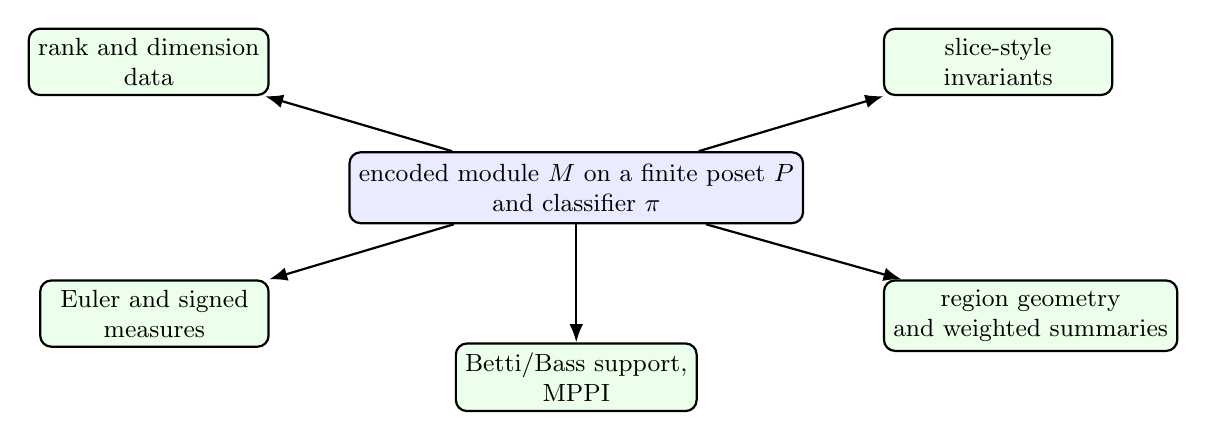
\begin{tikzpicture}[
  >=Latex,
  node distance=7mm and 10mm,
  every node/.style={font=\small},
  core/.style={rounded corners, draw, thick, align=center, minimum width=3.2cm, minimum height=0.9cm, fill=blue!8},
  fam/.style={rounded corners, draw, thick, align=center, minimum width=2.9cm, minimum height=0.8cm, fill=green!8}
]
\node[core] (enc) {encoded module $M$ on a finite poset $P$\\and classifier $\pi$};
\node[fam, above left=of enc] (rank) {rank and dimension\\data};
\node[fam, above right=of enc] (slice) {slice-style\\invariants};
\node[fam, below left=of enc] (euler) {Euler and signed\\measures};
\node[fam, below right=of enc] (geom) {region geometry\\and weighted summaries};
\node[fam, below=15mm of enc] (alg) {Betti/Bass support,\\MPPI};
\draw[->, thick] (enc) -- (rank);
\draw[->, thick] (enc) -- (slice);
\draw[->, thick] (enc) -- (euler);
\draw[->, thick] (enc) -- (geom);
\draw[->, thick] (enc) -- (alg);
\end{tikzpicture}

\medskip
\raggedright
The code therefore implements a \emph{family} of invariants and geometry-aware summaries,
all built from the same finite encoded object.
\end{frame}

\begin{frame}{Complete inventory by family I}
\scriptsize
\begin{tabularx}{\textwidth}{>{\raggedright\arraybackslash}p{2.8cm}X}
\toprule
Family & Implemented functions \\
\midrule
Rank and dimension & \texttt{restricted\_hilbert}, \texttt{rank\_map}, \texttt{rank\_invariant}, \texttt{rank\_invariant\_tame}, \texttt{ecc}, \texttt{hilbert\_distance} \\
Rectangle and rank inversion & \texttt{rectangle\_signed\_barcode}, \texttt{rectangle\_signed\_barcode\_rank}, \texttt{rank\_from\_signed\_barcode}, \texttt{truncate\_signed\_barcode}, \texttt{rectangle\_signed\_barcode\_image}, \texttt{rectangle\_signed\_barcode\_kernel}, \texttt{rectangle\_measure}, \texttt{rectangles} \\
Slice barcodes & \texttt{slice\_chain}, \texttt{restrict\_to\_chain}, \texttt{slice\_barcode}, \texttt{slice\_barcodes}, \texttt{slice\_chain\_exact\_2d}, \texttt{fibered\_slice}, \texttt{fibered\_slice\_family\_2d} \\
Slice distances & \texttt{bottleneck\_distance}, \texttt{wasserstein\_distance}, \texttt{sliced\_bottleneck\_distance}, \texttt{sliced\_wasserstein\_distance}, \texttt{sliced\_wasserstein\_distance\_approx}, \texttt{matching\_distance}, \texttt{matching\_distance\_approx}, \texttt{matching\_distance\_approx\_2d}, \texttt{matching\_distance\_exact\_2d}, \texttt{matching\_distance\_exact\_slices\_2d} \\
Slice features and kernels & \texttt{PersistenceLandscape1D}, \texttt{persistence\_landscape}, \texttt{PersistenceImage1D}, \texttt{persistence\_image}, \texttt{persistence\_silhouette}, \texttt{barcode\_entropy}, \texttt{barcode\_summary}, \texttt{slice\_features}, \texttt{slice\_kernel}, \texttt{wasserstein\_kernel} \\
Projected and fibered caches & \texttt{FiberedArrangement2D}, \texttt{FiberedBarcodeCache2D}, \texttt{fibered\_barcode}, \texttt{fibered\_barcode\_index}, \texttt{fibered\_values}, \texttt{ProjecteArrangement}, \texttt{ProjectedBarcodeCache}, \texttt{projected\_arrangement}, \texttt{projected\_barcode\_cache}, \texttt{projected\_barcodes}, \texttt{projected\_distances}, \texttt{projected\_distance}, \texttt{projected\_kernel} \\
\bottomrule
\end{tabularx}
\end{frame}

\begin{frame}{Complete inventory by family II}
\scriptsize
\begin{tabularx}{\textwidth}{>{\raggedright\arraybackslash}p{3.0cm}X}
\toprule
Family & Implemented functions \\
\midrule
Euler and signed measures & \texttt{euler\_characteristic\_surface}, \texttt{euler\_surface}, \texttt{euler\_signed\_measure}, \texttt{euler\_distance}, \texttt{PointSignedMeasure}, \texttt{point\_signed\_measure}, \texttt{surface\_from\_point\_signed\_measure}, \texttt{truncate\_point\_signed\_measure}, \texttt{point\_signed\_measure\_kernel} \\
Multiparameter landscape and image families & \texttt{MPLandscape}, \texttt{mp\_landscape}, \texttt{mp\_landscape\_distance}, \texttt{mp\_landscape\_inner\_product}, \texttt{mp\_landscape\_kernel}, \texttt{multiparameter\_landscape}, \texttt{multiparameter\_landscape\_standard}, \texttt{MPPLineSpec}, \texttt{MPPDecomposition}, \texttt{mpp\_decomposition}, \texttt{MPPImage}, \texttt{mpp\_image}, \texttt{mpp\_image\_distance}, \texttt{mpp\_image\_inner\_product}, \texttt{mpp\_image\_kernel}, \texttt{mma\_decomposition} \\
Weighted module summaries & \texttt{integrated\_hilbert\_mass}, \texttt{measure\_by\_dimension}, \texttt{measure\_by\_value}, \texttt{support\_measure}, \texttt{vertex\_set\_measure}, \texttt{region\_values}, \texttt{dim\_stats}, \texttt{dim\_norm}, \texttt{region\_weight\_entropy}, \texttt{aspect\_ratio\_stats}, \texttt{module\_size\_summary}, \texttt{module\_geometry\_summary} \\
Interface and graph summaries & \texttt{interface\_measure}, \texttt{interface\_measure\_by\_dim\_pair}, \texttt{interface\_measure\_dim\_changes}, \texttt{graph\_degrees}, \texttt{graph\_connected\_components}, \texttt{graph\_modularity}, \texttt{region\_adjacency\_graph\_stats}, \texttt{region\_volume\_samples\_by\_dim}, \texttt{region\_volume\_histograms\_by\_dim}, \texttt{region\_boundary\_to\_volume\_samples\_by\_dim}, \texttt{region\_boundary\_to\_volume\_histograms\_by\_dim} \\
Algebraic support descriptors & \texttt{betti\_support\_measures}, \texttt{bass\_support\_measures}, \texttt{upsets\_covering}, \texttt{downsets\_covering}, \texttt{minimal\_primes}, \texttt{socle}, \texttt{associated\_primes} \\
\bottomrule
\end{tabularx}
\end{frame}

\begin{frame}{Rank and dimension-type invariants}
\small
For an encoded finite-poset module $M$:
\begin{itemize}
  \item \textbf{Restricted Hilbert function}
  \[
    h_M(p)=\dim_{\kk} M_p.
  \]
  This is the dimension surface on the encoding poset.
  \item \textbf{Rank invariant}
  \[
    \rho_M(a,b)=\operatorname{rank}\bigl(M(a\le b)\bigr),\qquad a\le b.
  \]
  \item \textbf{Rectangle signed barcode / signed measure}

  On a finite grid, one may Mobius-invert the rank invariant to obtain a signed sum of rectangles.
  This is the multiparameter analog of turning cumulative rank data into local contributions.
\end{itemize}

\medskip
\textbf{Why this family matters.}
It is exact, finite-poset, and algebraic.  It is the starting point for rectangle images,
rank-from-signed-barcode recovery, and several later distances and kernels.
\end{frame}

\begin{frame}{Slice-style invariants}
\small
Choose a monotone chain or slice $\lambda$ in parameter space.  Restriction gives a 1-parameter module
\[
  \lambda^* M,
\]
and hence an ordinary barcode.

\medskip
\textbf{Primary objects}
\begin{itemize}
  \item \texttt{slice\_barcode}, \texttt{slice\_barcodes}
  \item fibered and projected caches for repeated slicing
  \item exact and approximate matching distance in 2D
\end{itemize}

\textbf{Derived 1D summaries on slices}
\begin{itemize}
  \item persistence landscape
  \item persistence image
  \item persistence silhouette
  \item barcode entropy and barcode summary
  \item sliced bottleneck and sliced Wasserstein distances
\end{itemize}

\end{frame}

\begin{frame}{Euler and signed-measure invariants}
\small
When the encoded object is a module or a cochain complex, the library also supports Euler-type data.

\begin{itemize}
  \item \textbf{Euler surface}
  \[
    \chi(x)=\sum_i (-1)^i \dim_{\kk} C^i(x)
  \]
  evaluated on a chosen grid or on axes induced by the encoding.
  \item \textbf{Euler signed measure}

  Mobius inversion of the Euler surface on the product-of-chains grid yields a sparse signed point measure.
  \item \textbf{Point signed measure kernels and distances}

  These convert the sparse signed measure into a reusable low-dimensional descriptor.
\end{itemize}

\end{frame}

\begin{frame}{Multiparameter landscapes and persistence images}
\small
There are two related image-like summary families.

\begin{itemize}
  \item \textbf{Slice-aggregated family:} \texttt{mp\_landscape}, plus the standard 1D
  landscape/image constructions applied slice-by-slice and aggregated.
  \item \textbf{Carriere-style family:}
  \texttt{mpp\_decomposition} and \texttt{mpp\_image}.
\end{itemize}

\medskip
\textbf{MPPI idea.}
The code stores a finite family of weighted line segments in the plane:
\[
  I_k \leadsto \{(p,q,\omega)\}_{\text{segments}}
\]
and then rasterizes them into an image by Gaussian smoothing.

\medskip
This gives:
\begin{itemize}
  \item a visual descriptor,
  \item an inner product / kernel,
  \item and a distance between images.
\end{itemize}

These are especially useful for machine learning workflows where one wants a stable, fixed-size representation.
\end{frame}

\begin{frame}{Geometry from PL encodings}
\small
For PL and box encodings, the classifier map carries actual region geometry.
This is not a separate invariant family in the narrow algebraic sense, but it is a major source of geometric summaries.

\medskip
\textbf{Region geometry API}
\begin{itemize}
  \item size and support: \texttt{region\_weights}, \texttt{region\_volume}, \texttt{region\_bbox}, \texttt{region\_widths}, \texttt{region\_diameter}
  \item shape: \texttt{region\_centroid}, \texttt{region\_aspect\_ratio}, \texttt{region\_principal\_directions}, \texttt{region\_covariance\_anisotropy}, \texttt{region\_covariance\_eccentricity}
  \item boundary and adjacency: \texttt{region\_adjacency}, \texttt{region\_boundary\_measure}, \texttt{region\_perimeter}, \texttt{region\_surface\_area}
  \item inscribed / circumscribed geometry: \texttt{region\_chebyshev\_ball}, \texttt{region\_inradius}, \texttt{region\_circumradius}
  \item integral summaries: \texttt{region\_boundary\_to\_volume\_ratio}, \texttt{region\_isoperimetric\_ratio}, \texttt{region\_mean\_width}, \texttt{region\_minkowski\_functionals}
\end{itemize}

\medskip
These data feed weighted invariants such as \texttt{support\_measure},
\texttt{integrated\_hilbert\_mass}, \texttt{aspect\_ratio\_stats},
\texttt{interface\_measure}, and \texttt{module\_geometry\_summary}.
\end{frame}

\begin{frame}{Algebraic support descriptors and takeaway}
\small
The implementation also includes algebraic support summaries that sit closer to commutative algebra:
\begin{itemize}
  \item \texttt{betti\_support\_measures}, \texttt{bass\_support\_measures}
  \item \texttt{minimal\_primes}, \texttt{socle}, \texttt{associated\_primes}
  \item covering summaries such as \texttt{upsets\_covering} and \texttt{downsets\_covering}
\end{itemize}

\medskip
\textbf{Takeaway.}
\begin{enumerate}
  \item The library does not implement a single ``multiparameter barcode.''
  \item It instead keeps the finite encoded module and exposes many invariant families.
  \item The right invariant depends on the question:
  \begin{itemize}
    \item rank and Hilbert data for exact algebraic structure,
    \item slices for 1D comparison matching distances, and similar
    \item Euler and signed measures for compact summaries,
    \item MPPI and landscapes for feature extraction,
    \item PL region geometry for weighted and geometric summaries.
  \end{itemize}
\end{enumerate}
\end{frame}

\end{document}
